\msection{Offensive Diversification: Malware evasion}

The primary malicious use of WebAssembly in browsers is cryptojacking \cite{musch2019new}. 
This is due to the essence of cryptojacking, the faster the mining, the better. 
Although the research of Lehmann and colleagues \cite{Hilbig2021AnES} suggests a decline in browser-based cryptominers, mainly due to the shutdown of Coinhive, a 2022 report by Kaspersky indicates that the use of cryptominers is on the rise \cite{kasperksy}. 
This underscores the ongoing need for effective automatic detection of cryptojacking malware.


Both antivirus software and browsers have implemented measures to detect cryptojacking. For instance, Firefox employs deny lists to detect cryptomining activities \cite{firefoxcrypto}. 
The academic community has also contributed to the body of work on detecting or preventing WebAssembly-based cryptojacking, as outlined in \autoref{background:wasm:analysis}. 
However, it's worth noting that malicious actors can employ evasion techniques to circumvent these detection mechanisms. 
Bhansali et al. are among the first who have investigated how WebAssembly cryptojacking could potentially evade detection \cite{10.1145/3507657.3528560}, highlighting the critical importance of this use case. 
For an in-depth discussion on this topic, we direct the reader to our contribution \cite{EVASION}.
The use of case illustrated in the subsequent sections uses Offensive Software Diversification for the sake of evading malware detection in \Wasm. 


\msubsection{Threat model: cryptojacking defense evasion}
\label{threat_model}

Let us illustrate the threat model in which a malicious \wasm binary could be involved.
\autoref{fig:attack_crypto} illustrates a browser attack scenario:
a practical WebAssembly cryptojacking attack consists of three components: a WebAssembly binary, a JavaScript wrapper, and a backend cryptominer pool. 
The WebAssembly binary is responsible for executing the hash calculations, which consume significant computational resources. 
The JavaScript wrapper facilitates the communication between the WebAssembly binary and the cryptominer pool.

\begin{figure}[h]
    \centering
    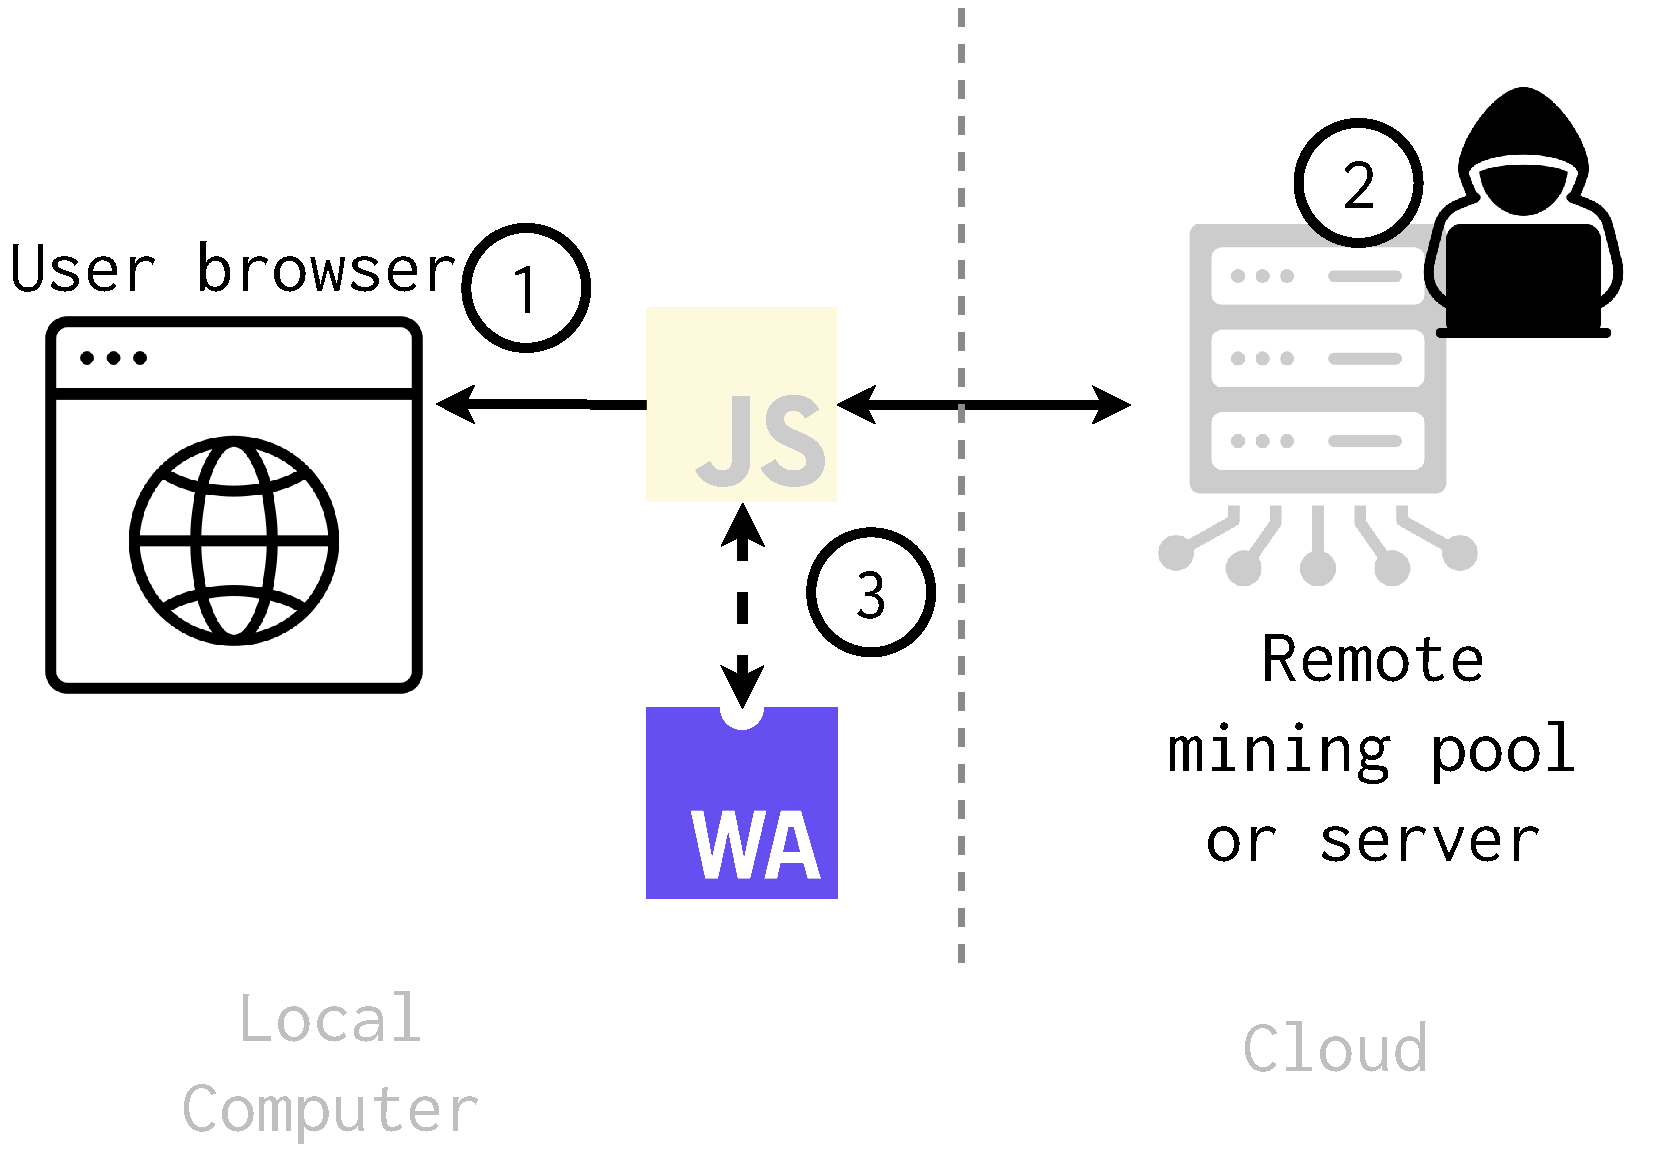
\includegraphics[width=0.6\linewidth]{figures/attack_crypto.pdf}
    \caption{Cryptojacking components.}
    \label{fig:attack_crypto}
\end{figure}

For the previous triad to work, the following steps are executed.
First, the victim visits a web page infected with the cryptojacking code. 
The web page establishes a channel to the cryptominer pool, which then assigns a hashing job to the infected browser. 
The WebAssembly cryptominer calculates thousands of hashes inside the browser. 
Once the malware server receives acceptable hashes, it is rewarded with cryptocurrencies for the mining. 
Then, the server assigns a new job, and the mining process starts over.

\begin{figure}
    \centering
    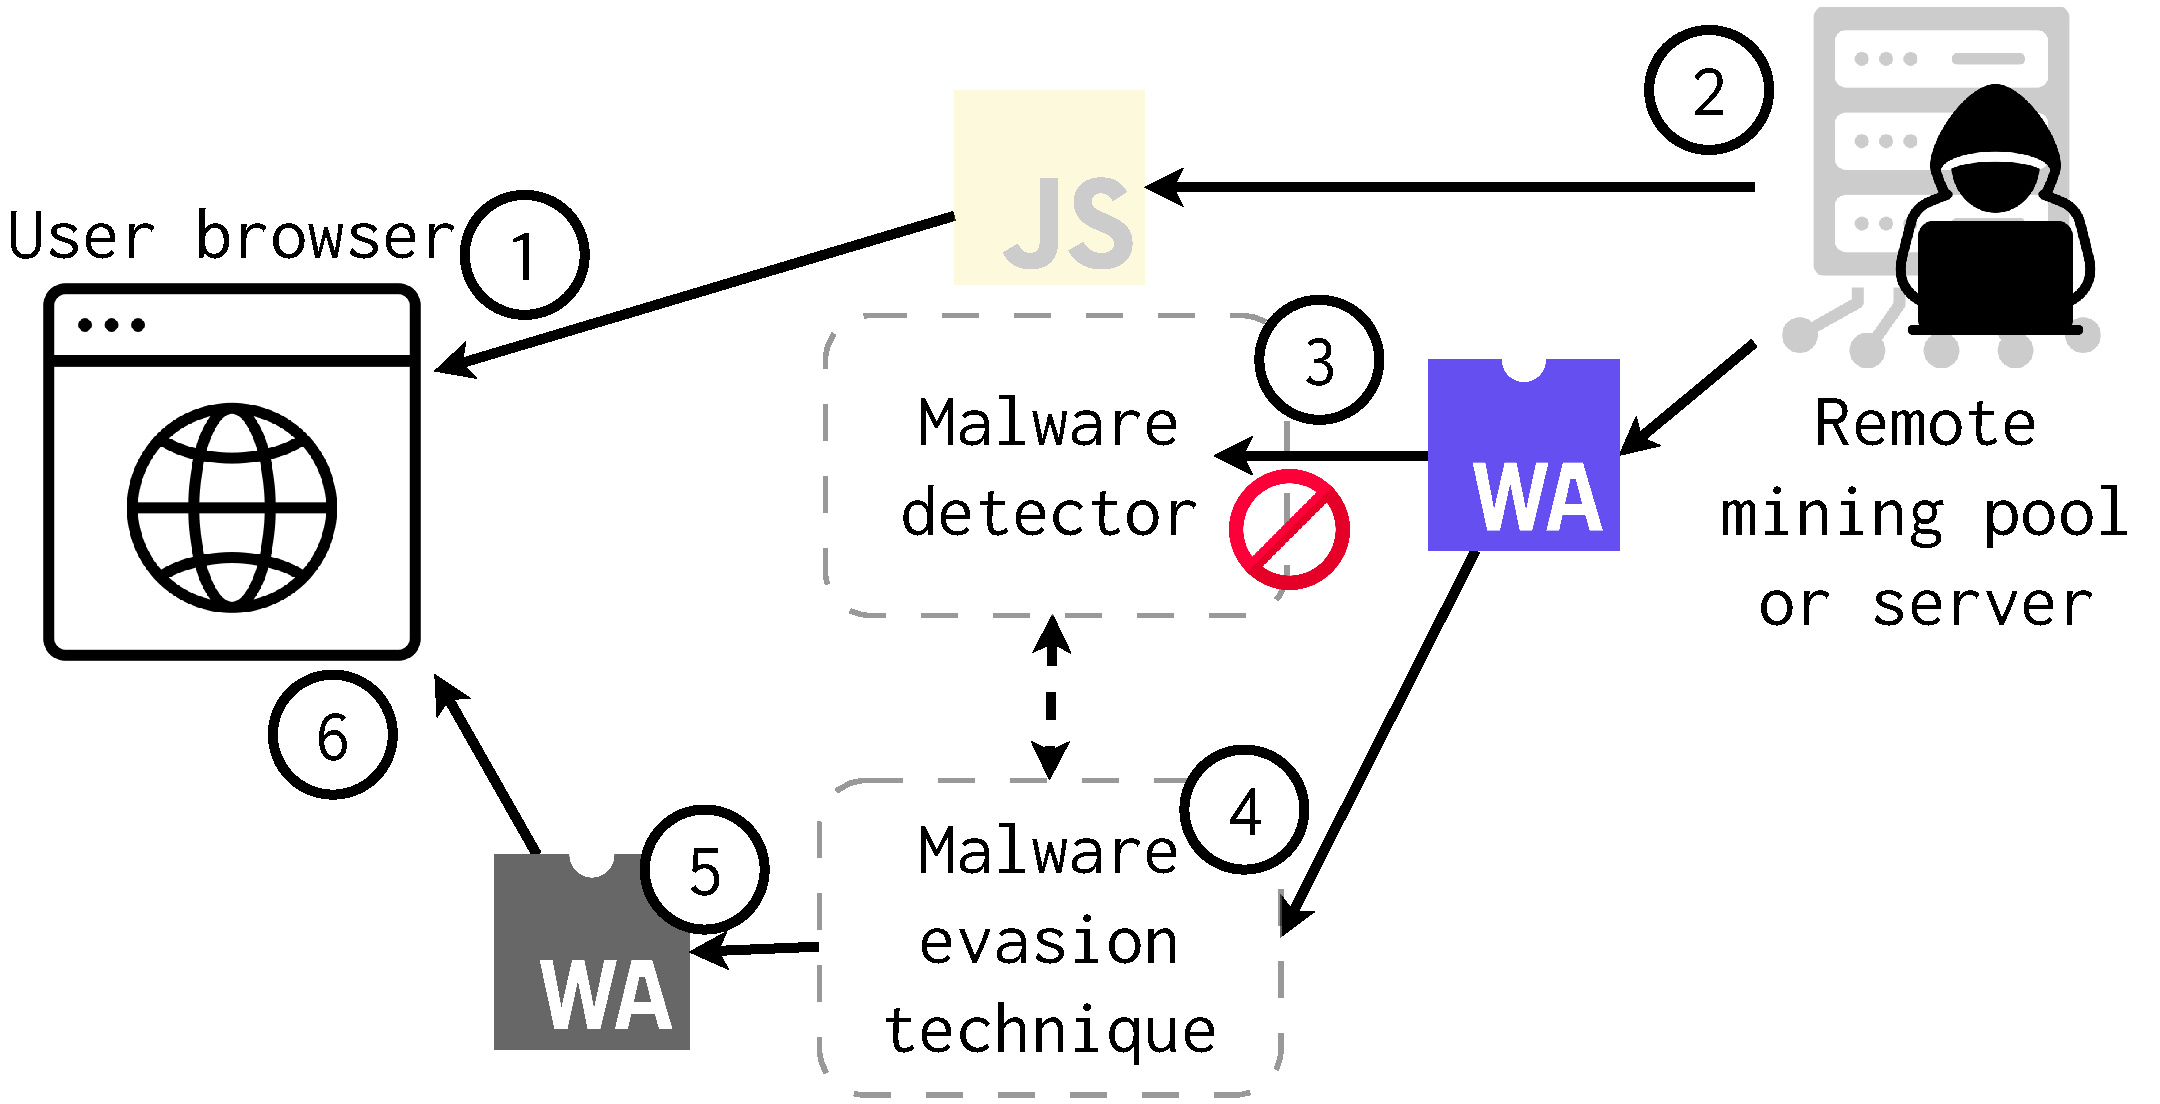
\includegraphics[width=0.8\linewidth]{figures/threat_model.pdf}
    \caption{Taken from \cite{EVASION}}
    \label{fig:threat_model}
\end{figure}


Considering the previous scenario, several techniques, as outlined in \autoref{background:wasm:analysis}, can be directly implemented in browsers to thwart cryptojacking by identifying the malicious \Wasm components. 
Such defense scenario is illustrated in \autoref{fig:threat_model}, where the \Wasm malicious binary is blocked in \step{3}.
The primary aim of our use of case is to investigate the effectiveness of code diversification as a means to circumvent cryptojacking defenses. 
Specifically, we assess whether the following evasion workflow can successfully bypass existing security measures:

\begin{enumerate}
    
    \item The user lands on a webpage infected with cryptojacking malware, which leverages network resources for execution—corresponding to \step{1} and \step{2} in \autoref{fig:threat_model}. 
    Notice that, various methods can be used to inject cryptojacking malware, including malicious browser extensions, malvertising, compromised websites, or deceptive links \cite{9566204}.
    
    \item A malware detection mechanism(malware oracle) identifies and blocks malicious WebAssembly binaries at \step{3}. 
    For example, a network proxy could intercept and forward these resources to an external detection service via its API.
    
    \item Anticipating that a specific malware detection system is consistently used for defense, the attacker swiftly generates a variant of the WebAssembly cryptojacking malware designed to evade detection at \step{4}.
    
    \item The attacker delivers the modified binary instead of the original one \step{5}, which initiates the cryptojacking process and compromises the browser \step{6}. The detection method is completely oblivious to the malicious nature of the binary, and the attack is successful.
    
\end{enumerate}


\msubsection{Methodology}

In this study, we categorize malware detection mechanisms as malware oracles, which can be of two types: binary and numeric. 
A binary oracle provides a binary decision, labeling a \Wasm binary as either malicious or benign. 
In contrast, a numeric oracle returns a numerical value representing the confidence level of the detection.

\begin{definition}{Malware oracle}
    \label{malware_oracle_def}
    A malware oracle is a detection mechanism that returns either a binary decision or a numerical value indicating the confidence level of the detection.
\end{definition}


For empirical validation, we employ VirusTotal as a numeric oracle and MINOS \cite{MINOS} as a binary oracle. 
VirusTotal is an online service that analyzes files and returns a confidence score, thus qualifying as a numeric oracle. 
MINOS, on the other hand, converts \Wasm binaries into grayscale images and employs a convolutional neural network for classification. 
It returns a binary decision, making it a binary oracle.


We use the wasmbench dataset \cite{Hilbig2021AnES} to establish a ground truth. 
After running the wasmbench dataset through VirusTotal and MINOS, we identify 33 binaries flagged as malicious by at least one VirusTotal vendor and also detected by MINOS.

To simulate the evasion scenario, we use WASM-MUTATE to generate \Wasm binary variants to evade malware detection.
We use WASM-MUTATE in two configurations: controlled and uncontrolled diversification.

\begin{definition}{Uncontrolled Diversification}
    \label{uncontrolled_def}
    Unlike controlled diversification, uncontrolled diversification is a stochastic process where each transformation has an equal likelihood of being applied to the input \Wasm binary.
\end{definition}

\begin{definition}{Controlled Diversification}
    \label{controlled_def}
    In controlled diversification, the transformation process of a \Wasm program is guided by a numeric oracle, which influences the probability of each transformation. For instance, WASM-MUTATE can be configured to apply transformations that minimize the oracle's confidence score. Note that controlled diversification needs a numeric oracle.
\end{definition}


Based on the two types of malware oracles and diversification configurations, we examine three scenarios:
1) VirusTotal with a controlled diversification, 2) VirusTotal with an uncontrolled diversification, and 3) MINOS with an uncontrolled diversification.
Notice that, the fourth scenario with MINOS and a controlled diversification is not feasible, as MINOS is a binary oracle and cannot provide the numerical values required for controlled diversification.

Our evaluation focuses on two key metrics: the success rate of evading detection mechanisms in VirusTotal and MINOS across the 33 flagged binaries, and the performance impact on the variants that successfully evade detection.
The first metric measures the efficacy of WASM-MUTATE in bypassing malware detection systems. 
For each flagged binary, we input it into WASM-MUTATE, configured with the selected oracle and diversification strategy. 
We then iteratively apply transformations to the output from the preceding step. 
This iterative process is halted either when the binary is no longer flagged by the oracle or when a maximum of 1000 stacked transformations have been applied.
This process is repeated with 10 random seeds per binary to simulate 10 different evasion experiments per binary.
The second metric is crucial for validating the real-world applicability of WASM-MUTATE in evading malware detection. 
Specifically, if the evasion process significantly degrades the performance of the resulting binary compared to its original version, it becomes less likely to be employed in practical scenarios, such as cryptojacking.

%\lipsum[1]

%\lipsum[1]

\msubsection{Evasion results}

\begin{comment}

                 24aae13a & 980.0 & 000415b2 & 960.0 \\
             59955b4c & 38.0  & 119c53eb & 1.0  \\
             fb15929f & 1.0  & 5bc53343 & 33.0  \\
             47d29959 & 100.0  & dc11d82d & 115.0  \\
             a27b45ef & 33.0  & 006b2fb6 & 1.0   \\
             942be4f7 & 29.0  & 7c36f462 & 85.0  \\
             0d996462 & 24.0  & 15b86a25 & 1.0  \\
             8ebf4e44 & 92.0  & a74a7cb8 & 38.0  \\
             fbdd1efa & 1.0  & 089dd312 & 68.0  \\
             65debcbe & 38.0  & aafff587 & 1.0  \\
             046dc081 & 33.0  & 6b8c7899 & 38.0  \\
             a32a6f4b & 1.0  & d2141ff2 & 81.0  \\
             68ca7c0e & 38.0  & dceaf65b & 66.0  \\
             9d30e7f0 & 419.0  & 4cbdbbb1 & 1.0  \\
             643116ff & 47.0  & c1be4071 & 38.0  \\
             e09c32c5 & 15.0  & f0b24409 & 33.0  \\
             89a3645c & 108.0 

\end{comment}

In \autoref{offensive:results:fast}, we present a comprehensive summary of the evasion experiments presented in \cite{EVASION}, focusing on two oracles: VirusTotal and MINOS\cite{MINOS}. The table is organized into two main categories to separate the results for each malware oracle. 
For VirusTotal, we further subdivide the results based on the two diversification configurations we employ: uncontrolled and controlled diversification. 
In these subsections, we provide columns that indicate the number of initial detections (\#D), the maximum number of successfully evaded detectors (Max. \#evaded), and the average number of transformations required (Mean \#trans.) for each sample. 
We highlight in bold text the values for which the uncontrolled diversification or controlled diversification setups are better than each other, the lower, the better.
The MINOS section simply includes a column that specifies the number of transformations needed for complete evasion. 
The table has 33 + 1 rows, each representing a unique \wasm malware study subject. 
The final row offers the median number of transformations required for evasion across all setups and oracles. 

\newcolumntype{t}{>{\columncolor{Gray}}r}
\begin{table}
    \footnotesize
    \centering
    \begin{tabular}{c | r | r l | r l | t }
        \hline
        & \multicolumn{5}{|c|}{VirusTotal} & MINOS\cite{MINOS} \\
        \hline
        Hash & \#D & \multicolumn{2}{c|}{Uncontrolled diversification} & \multicolumn{2}{c|}{Controlled diversification} & \\
        \hline
        &  & Max. #evaded & Mean #trans. & Max. #evaded & Mean #trans. & Mean #trans. \\
        \hline\hlined
        47d29959 &                 31 &             \textbf{26} &     N/A & 19 & N/A  & 100  \\ 
        9d30e7f0 &                 30 &             \textbf{24}  &      N/A & 17 & N/A & 419  \\ 
        8ebf4e44 &                 26 &             \textbf{21} &     N/A  & 13 & N/A & 92 \\
        \hline
        c11d82d &                 20 &       20        &  \textbf{355} & 20 & 446 & 115 \\ 
        0d996462 &                 19 &     19    &  \textbf{401} & 19 & 697 & 24 \\ 
        a32a6f4b &                 18 &       18       &  635 & 18 & \textbf{625} & 1 \\
        
        
        fbdd1efa &                 18 &         18      &  \textbf{310} & 18 & 726 & 1 \\ 
        d2141ff2 &                  9 &          9      &  \textbf{461} & 9 & 781 & 81 \\ 
        aafff587 &                  6 &          6      &  484 & 6 & \textbf{331} & 1 \\
        
        
        046dc081 &                  6 &          6      &  404 & 6 & \textbf{159} & 33 \\ 
        643116ff &                  6 &          6      &  \textbf{144} & 6 & 436 & 47 \\ 
        15b86a25 &                  4 &          4      &  253 & 4 & \textbf{131} & 1 \\
        
        
        
        006b2fb6 &                  4 &           4     &  \textbf{282} & 4 & 380 & 1\\ 
        942be4f7 &                  4 &           4     &  200 & 4 & 200 & 29\\ 
        7c36f462 &                  4 &           4     &  236 & 4 & \textbf{221} & 85\\
        
        
        fb15929f &                  4 &            4    &  \textbf{297} & 4 & 475 & 1 \\ 
        24aae13a &                  4 &         4       &  \textbf{252 } & 4 & 401 & 980\\ 
        000415b2 &                  3 &         3       &  302 & 3 & \textbf{34} & 960 \\
        
        4cbdbbb1 &                  3 &          3      &  295 & 3 & \textbf{72} & 1\\ 
        65debcbe &                  2 &          2      &  131  & 2 & \textbf{33} & 38 \\ 
        59955b4c &                  2 &          2      &  130  & 2 & \textbf{33} & 38 \\
        
        
        89a3645c &                  2 &           2     &  431 & 2 & \textbf{107} & 108\\
        a74a7cb8 &                  2 &           2     &  124 & 2 & \textbf{33} & 38 \\
        119c53eb &                  2 &           2     &  104 & 2 & \textbf{18} & 1 \\
        
        089dd312 &                  2 &           2     &  153 & 2 & \textbf{123} & 68\\
        c1be4071 &                  2 &           2     &  130 & 2 & \textbf{33} & 38\\
        dceaf65b &                  2 &           2     &  140 & 2 & 132 & 66\\
        
        6b8c7899 &                  2 &            2    &  143 & 2 & \textbf{33} & 38 \\
        a27b45ef &                  2 &         2       &  145 & 2 & \textbf{33} & 33\\
        68ca7c0e &                  2 &         2       &  137  & 2 & \textbf{33} & 38\\
        
        f0b24409 &                  2 &         2       &  127  & 2 & \textbf{11} & 33 \\
        5bc53343 &                  2 &         2       &  118  & 2 & \textbf{33} & 33 \\
        e09c32c5 &                  1 &         1       &  \textbf{120}  & 1 & 488 & 15 \\
        \hline\hline
        Median &                         &         &      218  &   & 131 & 38
    \end{tabular}
    \caption{TODO description and main takeaway}
    \label{offensive:results:fast}
\end{table}


\wrule{Uncontrolled diversification to evade VirusTotal:} We run uncontrolled diversification with WASM-MUTATE with a limit of 1000 iterations per binary. 
At each iteration, we query VirusTotal to check if the new binary evades the detection.
This process is repeated with 10 random seeds per binary to simulate 10 different evasion experiments per binary.
As shown in the uncontrolled diversification part of \autoref{offensive:results:fast}, we successfully generate variants that evade detection for 30 out of 33 binaries.
The mean value of iterations needed to generate a variant that evades all detectors ranges from 120 to 635 stacked transformations.
The mean number of iterations needed is always less than 1000 stacked transformations.
There are 3 binaries for which the uncontrolled diversification setup does not completely evade the detection. 
In these three cases, the algorithm misses 5 out 31, 6 out of 30 and 5 out 26 detectors.
The explanation is the maximum number of iterations 1000 we use for our experiments.
However, having more iterations seems not a realistic scenario.
For example, if some transformations increment the binary size during the transformation, a considerably large binary might be impractical for bandwidth reasons.
Overall, uncontrolled diversification with WASM-MUTATE clearly decreases the detection rate by VirusTotal antivirus vendors for cryptojacking malware, achieving total evasion of WebAssembly cryptojacking malware in 30/33 (90\%) of the malware dataset.
When compared with the data in \autoref{comp:table:tools}, it becomes evident that WASM-MUTATE generates an average of nearly 10000 variants per binary within an hour. 
Thus, WASM-MUTATE is capable of successfully evading detection systems in just a matter of minutes.

\wrule{Controlled diversification to evade VirusTotal:}  Uncontrolled diversification does not guide the diversification based on the number of evaded detectors, it is purely random, and has some drawbacks.
For example, some transformations might suppress other transformations previously applied.
We have observed that, by carefully selecting the order and type of transformations applied, it is possible to evade detection systems in fewer iterations.
This can be appreciated in the results of the controlled diversification part of \autoref{offensive:results:fast}.
Analyzing the data in \autoref{offensive:results:fast}, we observe that the controlled diversification setup successfully generates variants that totally evade the detection for 30 out of 33 binaries, it thus as good as the uncontrolled setup.
The iterations needed for the controlled diversification setup are 92\% of the needed on average for the uncontrolled diversification setup.
% The best cases
For 21 of 30 binaries that evade detection entirely, we observe that the mean number of oracle calls needed is lower than those in the baseline evasion algorithm.
For example, \texttt{f0b24409} needs 11 oracle calls with controlled diversification setup to fully evade VirusTotal, while for the uncontrolled one, it needs 127 oracles calls.
For those 21 binaries, it needs only 40\% of the calls the controlled diversification setup needs.

\wrule{Uncontrolled diversification to evade MINOS: }Additionally, relying solely on VirusTotal as the detection mechanism could be problematic, especially when specialized solutions exist exclusively for \Wasm, unlike the general-purpose vendors in VirusTotal. 
To address this, we also assessed the efficacy of our evasion algorithms against MINOS, a \Wasm-specific antivirus. 
We iteratively applied random mutations to the original malware binary until either MINOS was fully evaded or a maximum iteration limit was reached. 
This process was repeated 10 times for each binary. 
The outcomes are displayed in the last column of \autoref{offensive:results:fast}.
The last row of \autoref{offensive:results:fast} shows that WebAssembly diversification requires fewer iterations to evade MINOS than VirusTotal, meaning that it is easier to evade MINOS.
The median number of iterations needed overall for evading VirusTotal is 218 for the uncontrolled diversification setup, and 131 for the controlled diversification setup, while for MINOS is 38.
Remarkably, WASM-MUTATE totally evades detection for 8 out of 33 binaries in one single iteration in the case of MINOS.
This shows that the MINOS model is fragile wrt binary diversification. 
According to those results, VirusTotal can be considered better than MINOS wrt to cryptojacking detection. 
The main reason is that a wider spectrum of antivirus vendors is used in VirusTotal, while MINOS is a single detector.

\msubsection{Efficiency and correctness results}

To measure the practical applications of WASM-MUTATE in evading malware detection, we select the six binaries we can build and execute end-to-end, because we have access to the three components annotated in \autoref{fig:attack_crypto}.
For those six binaries, we are able to replace the original WebAssembly binary with variants generated by our evasion methods. 
We execute the original binary and the variants generated by the baseline and MCMC evasion algorithms. 
The essence of a cryptojacking is to generate hashes at high-speed. 
Consequently, we assess the correctness of the variants concerning two properties: validity of the hashes and frequency of hash generation. 
  
  \autoref{tab:rq3} summarizes the key data for RQ3.
  Each row of the table corresponds to one binary that can be executed end-to-end, by reproducing the three components mentioned in \autoref{background:crypto}.
  The first two values of each row are the original binary's identifier and its original frequency of hash generation.
  Then, for our baseline algorithm, each row has the data for \rev{10} variants generated during a successful oracle evasion.
  For each one of the variants, we include the correctness percentage and the hashes calculated per second.
  The last group of columns of the table contains the correctness percentage and the hashes calculated per second for the \rev{10} variants generated with the MCMC algorithm.
  After each frequency of hashing measurement, we indicate the relative difference with the original frequency in parentheses.
  A difference larger or equal to 1.0 means that the variant is faster or as efficient as the original. On the contrary, the variant is slower if the difference is lower than 1.0.
  The table contains the information for 120 variants.
  

% All behave identically
We use the backend miner pools (see \autoref{background:crypto}) of the six cryptojacking to determine the validity of the hashes computed by all the programs.
All correctness assessments for the \rev{120} variants indicate that the miner pools do not detect any invalid hash when executing the WebAssembly cryptominer variants.
This means that the variants synthesized by the baseline and the MCMC algorithms to evade the malware oracle can still systematically generate valid hashes. 


% Efficiency
We have observed that \rev{23 of 120} variants are more efficient than the original cryptojacking.
For example, for the \texttt{fbdd1efa} binary, all its variants are from 1.27 to 1.43 faster than the original hash generation frequency.
This phenomenon occurs because WASM-MUTATE can perform transformations in the executable code, which work as optimizations.
Our experiments have revealed two sources of faster WebAssembly variants: loop unrolling transformations and code replacements that lead to smaller binaries. 
We have also found that debloating transformations, which remove unneeded structures and dead code, results in more hashes being produced by the cryptominer in the first few seconds of mining, likely because of faster compilation.

In summary, all this is evidence that focused optimization is a good primitive for evasion. 
% The contrary case.
On the contrary, \rev{97 out of 120} variants underperform compared to the original binary.
The worst case is the binary \texttt{0d996462}.
Its slowest variant has \rev{0.20} of the original generation frequency.
The main reason is that WASM-MUTATE also introduces non-optimal transformations regarding performance.

The variants generated by the baseline evasion algorithm tend to be slower than the MCMC evasion algorithm.
The MCMC evasion algorithm triggers fewer oracle calls and can generate variants faster than the ones generated by the evasion algorithm.
This phenomenon is a direct consequence of the MCMC evasion algorithm implementation, which has a selective strategy when applying transformations on a binary  (see \autoref{alg:mcmc}).
In summary, the MCMC evasion algorithm produces variants that fully evade the VirusTotal oracle with lower performance overhead during execution. The worst performant variant is only 1.93 times slower for the MCMC evasion algorithm.


% Instantiate with one binary
In \autoref{plot:distrib}, we plot the distribution of the hashes per second for variants generated for the  \texttt{fbdd1efa} cryptojacking.
In the figure, we include the original binary (in blue), the ten variants generated by the baseline algorithm (in orange), and the ten variants generated by the MCMC evasion algorithm (in green). 
Each violin plot corresponds to the hashes per second.
We observe a normal distribution around the exact number of hashes per second. 
In this case, we have observed that the MCMC evasion algorithm provides a hash-per-second ratio better than the original.
This phenomenon can be observed in the lines inside the violin plots, the green line is shifted to the right compared to the lines of the blue violin plot.

\begin{tcolorbox}[boxrule=1pt,arc=.3em,boxsep=-1.3mm]
  \textbf{Answer to RQ3}: 
   Our algorithms synthesize WebAssembly cryptojacking variants that fully evade our malware oracle and that provide the same functionality as the original. The execution of evading malware systematically produces valid hashes, and the variations in performance are imperceptible. For 19\% of the generated
variants, we observe better performance, and in the
worst case, the generated variant underperforms by five
times the original binary.
\end{tcolorbox}





\renewcommand\arraystretch{1.2}
\begin{adjustbox}{width=1\linewidth}
\rev{
  \begin{tabular}{c c | cr  cr  cr || cr  cr  cr}

        \toprule
           Hash &  Original h/s & \multicolumn{6}{c||}{Baseline algorithm} & \multicolumn{6}{c}{MCMC algorithm} \\
         \hline


        0d996462  &  116.0     &  100\%  & 25 (0.22)   &  100\%  & 24 (0.21)   &  100\%  & 26 (0.22)    &  100\%  & 116 \textbf{(1.00)}    &  100\%  & 70 (0.60)   &  100\%  & 67 (0.58)  \\ &    &  100\%  & 116 \textbf{(1.00)}    &  100\%  & 110 (0.95)   &  100\%  & 30 (0.26)    &  100\%  & 110 (0.95)   &  100\%  & 76 (0.66)   &  100\%  & 60 (0.52)  \\ &    &  100\%  & 55 (0.47)   &  100\%  & 27 (0.23)   &  100\%  & 23 (0.20)    &  100\%  & 86 (0.74)   &  100\%  & 60 (0.52)   &  100\%  & 72 (0.62)  \\ &    &  100\%  & 27 (0.23)    &   &   &   &   &   100\%  & 76 (0.66)  \\
        \hline
 a32a6f4b  &  48.0   &   100\%  & 25 (0.52)   &  100\%  & 24 (0.50)   &  100\%  & 24 (0.50)    &  100\%  & 26 (0.54)   &  100\%  & 45 (0.94)   &  100\%  & 41 (0.85)  \\ &    &  100\%  & 26 (0.54)   &  100\%  & 25 (0.52)   &  100\%  & 26 (0.54)    &  100\%  & 46 (0.96)   &  100\%  & 41 (0.85)   &  100\%  & 45 (0.94)  \\ &    &  100\%  & 26 (0.54)   &  100\%  & 24 (0.50)   &  100\%  & 25 (0.52)    &  100\%  & 44 (0.92)   &  100\%  & 42 (0.88)   &  100\%  & 45 (0.94)  \\ &    &  100\%  & 23 (0.48)    &   &  &  &  &  100\%  & 45 (0.94)  \\
        \hline
 fbdd1efa  &  37.0     &  100\%  & 25 (0.68)   &  100\%  & 25 (0.68)   &  100\%  & 25 (0.68)    &  100\%  & 28 (0.76)   &  100\%  & 47 \textbf{(1.27)}    &  100\%  & 48 \textbf{(1.30)}   \\ &    &  100\%  & 25 (0.68)   &  100\%  & 26 (0.70)   &  100\%  & 26 (0.70)    &  100\%  & 47 \textbf{(1.27)}    &  100\%  & 47 \textbf{(1.27)}    &  100\%  & 53 \textbf{(1.43)}   \\ &    &  100\%  & 25 (0.68)   &  100\%  & 25 (0.68)   &  100\%  & 25 (0.68)    &  100\%  & 48 \textbf{(1.30)}    &  100\%  & 48 \textbf{(1.30)}    &  100\%  & 49 \textbf{(1.32)}   \\ &    &  100\%  & 25 (0.68)     &   &  &  &   &  100\%  & 47 \textbf{(1.27)}   \\
        \hline
   d2141ff2  &  113.0    &  100\%  & 54 (0.48)   &  100\%  & 55 (0.49)   &  100\%  & 55 (0.49)    &  100\%  & 107 (0.95)   &  100\%  & 107 (0.95)   &  100\%  & 107 (0.95)  \\ &    &  100\%  & 57 (0.50)   &  100\%  & 56 (0.50)   &  100\%  & 56 (0.50)    &  100\%  & 109 (0.96)   &  100\%  & 106 (0.94)   &  100\%  & 100 (0.88)  \\ &    &  100\%  & 57 (0.50)   &  100\%  & 53 (0.47)   &  100\%  & 53 (0.47)    &  100\%  & 101 (0.89)   &  100\%  & 100 (0.88)   &  100\%  & 107 (0.95)  \\ &    &  100\%  & 55 (0.49)     &   &  &  &   &  100\%  & 107 (0.95)  \\
        \hline
   046dc081  &  118.0    &  100\%  & 58 (0.49)   &  100\%  & 60 (0.51)   &  100\%  & 59 (0.50)    &  100\%  & 118 \textbf{(1.00)}    &  100\%  & 120 \textbf{(1.02)}    &  100\%  & 119 \textbf{(1.01)}   \\ &    &  100\%  & 60 (0.51)   &  100\%  & 55 (0.47)   &  100\%  & 62 (0.53)    &  100\%  & 120 \textbf{(1.02)}    &  100\%  & 116 (0.98)   &  100\%  & 120 \textbf{(1.02)}   \\ &    &  100\%  & 55 (0.47)   &  100\%  & 50 (0.42)   &  100\%  & 57 (0.48)    &  100\%  & 119 \textbf{(1.01)}    &  100\%  & 120 \textbf{(1.02)}    &  100\%  & 119 \textbf{(1.01)}   \\ &    &  100\%  & 55 (0.47)     &   &  &  &   &  100\%  & 120 \textbf{(1.02)}   \\
        \hline
   006b2fb6  &  8.0    &  100\%  & 7 (0.88)   &  100\%  & 6 (0.75)   &  100\%  & 4 (0.50)    &  100\%  & 6 (0.75)   &  100\%  & 6 (0.75)   &  100\%  & 6 (0.75)  \\ &    &  100\%  & 9 \textbf{(1.12)}    &  100\%  & 6 (0.75)   &  100\%  & 4 (0.50)    &  100\%  & 6 (0.75)   &  100\%  & 6 (0.75)   &  100\%  & 6 (0.75)  \\ &    &  100\%  & 4 (0.50)   &  100\%  & 6 (0.75)   &  100\%  & 4 (0.50)    &  100\%  & 8 \textbf{(1.00)}    &  100\%  & 9 \textbf{(1.12)}    &  100\%  & 6 (0.75)  \\ &    &  100\%  & 6 (0.75)     &   &  &  &  &  100\%  & 6 (0.75)  \\
        \hline
    
        
    \end{tabular}
}
\end{adjustbox}




Remarkably, we find 30 cryptominers for which our technique successfully generates variants that evade VirusTotal.
Our set of malware includes 6 cryptojacking programs that are fully reproducible in a controlled environment. 
With them, we assess that our evasion method does not affect malware correctness and generates fully functional malware variants with minimal overhead.

Our work provides evidence that the malware detection community has opportunities to strengthen the automatic detection of cryptojacking WebAssembly malware. 
The results of this work are actionable, as we provide quantitative evidence on specific malware transformations on which detection methods can focus.


\begin{tcolorbox}[title=Contribution paper,boxrule=1pt,arc=.2em,boxsep=1.0mm]
    The case discussed in this section is fully detailed in Cabrera-Arteaga \etal "WebAssembly Diversification for Malware Evasion"
    \emph{at Computers \& Security, 2023}
    \url{https://www.sciencedirect.com/science/article/pii/S0167404823002067}. 
\end{tcolorbox}
